\documentclass[11pt, a4paper, lithuanian]{article}

\usepackage[left=25mm,right=15mm,top=15mm,bottom=15mm]{geometry}
\usepackage[utf8x]{inputenc}
\usepackage[L7x]{fontenc}
\usepackage[lithuanian]{babel}
\usepackage{listings}
\usepackage{amsmath, amssymb}
\usepackage{graphicx}
\usepackage{url}
\usepackage{subcaption}

\author{AKSfm-15, Maksim Norkin}
\title{Žinių inžinerija\\Pirmas labaoratorinis darbas}

\lstset{language=Matlab,
  basicstyle=\footnotesize,
  columns=fixed,
  numbers=none,
  showspaces=false,
  xleftmargin=20pt
}

\begin{document}

    \maketitle

    \section{Užduotis}

    Sukurti ekspertinę sistemą produkcijų sistemos \textit{STRESS} pagalba. Darbo metu buvo susipažinta su programine aplinka. Dalykinė sritis pasirinkta yra -- ``Kada daryti laboratorinį darbą''.

    \section{Atliktas darbas}

    Darbo metu buvo sukurti du objektai: ``DALYKAS'' ir ``ZMOGUS'', kiekvienas su savo atributais, kurie yra pateikti \ref{code:dalykas_atributai} ir \ref{code:zmogus_atributai} pavyzdžiuose.

    \begin{figure}
      \centering
      \lstinputlisting{sources/dalykas_atributai.text}
      \caption{``DALYKAS'' atributai}
      \label{code:dalykas_atributai}
    \end{figure}

    \begin{figure}
      \centering
      \lstinputlisting{sources/zmogus_atributai.text}
      \caption{``ZMOGUS'' atributai}
      \label{code:zmogus_atributai}
    \end{figure}

    Kiekvienas iš aprašytų atributų yra naudojamas žinių sistemos nuspręsti kada geriausia yra darytų dalyko namų darbą, turint duotą informaciją. Naudotojo lango iliustracija yra pateikiama \ref{img:sprendziamas_uzdavinys} pav.

    Paleidus programinį paketą, sistema pradžioje paklausia dviejų svarbiausių klausimų, kurie yra įvesti kaip forma \ref{img:pirminiu_klausimu_forma} pav. 

    Tolimesnis darbas yra informacijos apie objektų atributų vertes surinkimas. Vienas iš tokių atributų yra \textit{boolean} tipo atributas. Tokio atributo klausimo formos pavyzdys yra pateikiamas \ref{img:klausimas} pav.

    Kai sistema, remiantis taisyklių rinkiniu, pasiekia tam tikrą išvadą su užtikrintumo lygiu -- pateikiamas atsakymas \ref{img:atsakymas} pav.

    \begin{figure}
      \centering
      \begin{subfigure}[b]{0.45\textwidth}
        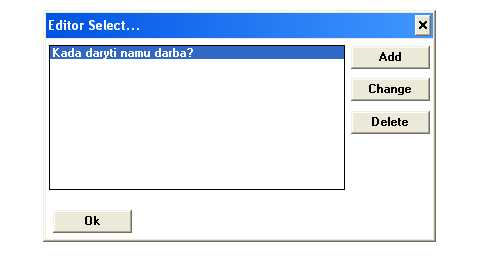
\includegraphics[height=130px]{img/sprendziamas_uzdavinys.png}
        \caption{Sprendžiamo uždavinio langas}
        \label{img:sprendziamas_uzdavinys}
      \end{subfigure}
      \begin{subfigure}[b]{0.45\textwidth}
        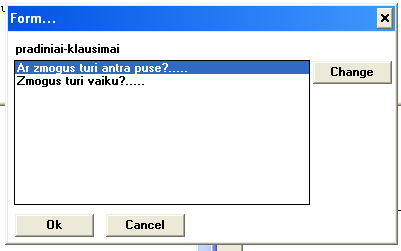
\includegraphics[height=130px]{img/forma.png}
        \caption{Sistemos pateikiama pirminių klausimų forma}
        \label{img:pirminiu_klausimu_forma}
      \end{subfigure}
      \caption{Sistemos veikimo iliustracijos}
    \end{figure}

    \begin{figure}
      \centering
      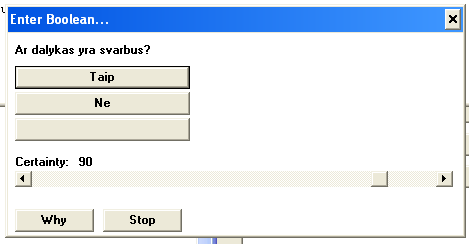
\includegraphics[width=0.45\textwidth]{img/klausimas.png}
      \caption{Sistemos pateikiamas klausimas}
      \label{img:klausimas}
    \end{figure}

    \begin{figure}
      \centering
      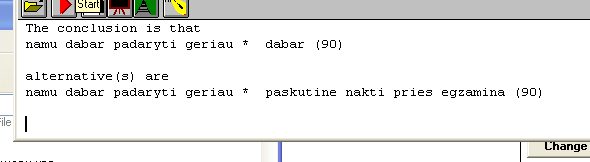
\includegraphics[width=\textwidth]{img/atsakymas.png}
      \caption{Sistemos pateikiamas atsakymas}
      \label{img:atsakymas}
    \end{figure}

    \section{Išvados}

    Laboratorinio darbo metu buvo išnagrinėtas \textit{STRESS} programinio paketo aplinka ir sukurta žinių sistema, su dviem objektais, jų atributais ir 25 klausimais, kurių tikslas yra prieiti prie užduoto uždavinio sprendimo, apklausinėjant naudotoją.

\end{document}
